\documentclass[11pt]{article}

% ===================== PACKAGES =====================
\usepackage[margin=1.15in]{geometry}
\usepackage{microtype}
\usepackage{amsmath, amssymb, amsthm, mathtools}
\usepackage{bm}
\usepackage{bbm}          % indicator 1_A
\usepackage{graphicx}     % figures
\usepackage{hyperref}     % links
\usepackage{amsmath}
\usepackage{algorithm}
\usepackage{algpseudocode}
\usepackage{booktabs} % for \toprule, \midrule, etc.
\usepackage{placeins} % for \FloatBarrier
\usepackage[numbers,sort&compress]{natbib}
\usepackage{caption}
\usepackage{xcolor}
\usepackage{listings}
\definecolor{codebg}{RGB}{245,245,245}
\definecolor{pygreen}{RGB}{0,128,0}
\definecolor{pyred}{RGB}{180,0,0}
\definecolor{pyblack}{RGB}{0,0,0}

\lstdefinestyle{pythonstyle}{
    language=Python,
    backgroundcolor=\color{codebg},
    basicstyle=\ttfamily\small\color{pyblack},
    keywordstyle=\color{blue},
    commentstyle=\color{pygreen},
    stringstyle=\color{pyred},
    showstringspaces=false,
    breaklines=true,
    frame=single,
    columns=fullflexible,
    keepspaces=true
}

\lstset{style=pythonstyle}

\usepackage{graphicx}
\usepackage{subcaption}
% Optional, only if you want to force figure placement with [h]
\usepackage{float}
\hypersetup{
  colorlinks=true,
  linkcolor=blue,
  citecolor=blue,
  urlcolor=blue
}

% ===================== SHORT COMMANDS =====================
% Sets / numbers
\newcommand{\R}{\mathbb{R}}
\newcommand{\N}{\mathbb{N}}
\newcommand{\Z}{\mathbb{Z}}
\newcommand{\T}{\mathbb{T}}

% Probability
\renewcommand{\P}{\mathbb{P}}
\newcommand{\E}{\mathbb{E}}
\DeclareMathOperator{\Var}{Var}
\DeclareMathOperator{\Cov}{Cov}

% Calculus / operators
\newcommand{\1}{\mathbbm{1}}
\newcommand{\dd}{\,\mathrm{d}}
\newcommand{\dt}{\,\mathrm{d}t}
\newcommand{\dW}{\,\mathrm{d}W}
\newcommand{\dB}{\,\mathrm{d}B}
\newcommand{\grad}{\nabla}
\newcommand{\Div}{\nabla\cdot}
\newcommand{\Tr}{\mathrm{Tr}}

% Vectors / matrices
\newcommand{\vv}[1]{\bm{#1}}
\newcommand{\mc}[1]{\mathcal{#1}}

% Convenience for long filenames
\newcommand{\BoffiPDF}{boffi-vanden-eijnden-2024-deep-learning-probability-flows-and-entropy-production-rates-in-active-matter.pdf}

% ===================== THEOREM ENVIRONMENTS =====================
\theoremstyle{plain}
\newtheorem{theorem}{Theorem}[section]
\newtheorem{lemma}[theorem]{Lemma}
\newtheorem{proposition}[theorem]{Proposition}
\newtheorem{corollary}[theorem]{Corollary}

\theoremstyle{definition}
\newtheorem{definition}[theorem]{Definition}
\newtheorem{assumption}[theorem]{Assumption}

\theoremstyle{remark}
\newtheorem{remark}[theorem]{Remark}

% ===================== DOCUMENT =====================
\title{SDE Project MATH 214}
\author{(Johan Jönsson)}
\date{\today}

\begin{document}
\maketitle

\tableofcontents
\newpage

% ============================================================
\section{Introduction to general model}
% ============================================================
This section introduces the active matter model that serves as the starting point for the project. The goal is to study a simplified version of the dynamics from \citet{boffi2024deep} and to investigate how physically meaningful constraints can be incorporated into both the continuous-time model and its numerical simulation. In particular, the aim is to construct and analyze a model in which the particle dynamics remain consistent with the intended physical behavior while still being simple enough to study mathematically and computationally.

% NOTE:
% - This includes the full PDF page where Fig. 2 appears.
% - If you want only the figure, crop using trim/clip, or export Fig. 2 as a separate image.

\subsection{Active Ornstein--Uhlenbeck / Gaussian colored-noise model}
Following \citet{boffi2024deep}, consider $N$ interacting self-propelled particles in dimension $d$ with
translational variables $x_t^i \in \R^d$ and orientational variables $g_t^i \in \R^d$.
Their dynamics is (Eq.\ (1) in the paper):
\begin{align}
\dot{x}_t^i
&=
\mu\sum_{j\neq i} f\bigl(x_t^i - x_t^j\bigr) + v_0 g_t^i + \sqrt{2\varepsilon}\,\xi_x^i(t),
\label{eq:boffi-eq1-x}\\
\dot{g}_t^i
&=
-\gamma g_t^i + \sqrt{2\gamma}\,\xi_g^i(t),
\label{eq:boffi-eq1-g}
\end{align}
for $i=1,\dots,N$. Here $\mu$ is the mobility, $f$ is a short-range repulsive force,
$v_0\ge 0$ is the self-propulsion speed, $\varepsilon\ge 0$ sets the thermal noise scale,
and $\gamma>0$ tunes the persistence timescale of self-propulsion.

The noises $\{\xi_x^i(t)\}$ and $\{\xi_g^i(t)\}$ are independent Gaussian white noises with
\[
\E\bigl[\xi_x^i(t)\xi_x^j(t')^\top\bigr] = \delta(t-t')\,\delta_{ij}\,I_d,
\qquad
\E\bigl[\xi_g^i(t)\xi_g^j(t')^\top\bigr] = \delta(t-t')\,\delta_{ij}\,I_d,
\]
and cross-covariances equal to $0$.

\subsection{Translation into It\^o SDE notation (probability-theory convention)}
White noise is the formal time-derivative of Brownian motion. Thus, introduce independent $d$-dimensional
Brownian motions $\{W_t^{x,i}\}_{i=1}^N$ and $\{W_t^{g,i}\}_{i=1}^N$ and rewrite
\eqref{eq:boffi-eq1-x}--\eqref{eq:boffi-eq1-g} as the It\^o system
\begin{align}
dX_t^i
&=
\Bigl(\mu\sum_{j\neq i} f\bigl(X_t^i - X_t^j\bigr) + v_0 G_t^i\Bigr)\dt
+ \sqrt{2\varepsilon}\,dW_t^{x,i},
\label{eq:ito-x}\\
dG_t^i
&=
(-\gamma G_t^i)\dt + \sqrt{2\gamma}\,dW_t^{g,i}.
\label{eq:ito-g}
\end{align}
This is the standard It\^o form used in texts like \citet{oksendal2013sde}. 

\subsection{Only repulsion}
We will now work with the case where we only have repulsion between particles which is defined using It\^o SDE notation the following way
\begin{align}
dX_t^i
&=
\Bigl(\mu\sum_{j\neq i} f\bigl(X_t^i - X_t^j\bigr) \Bigr)\dt
+ \sqrt{2\varepsilon}\,dW_t^{x,i}
\label{eq:ito-x-reponly}
\end{align}
We will now analyze the case where $N=2$ and $X_t^i \in \R$. Whcih gives the following equation
\begin{align}
\begin{bmatrix}
dX_t^1 \\
dX_t^2
\end{bmatrix} = \mu \begin{bmatrix}
f( X_t^1-X_t^2) \\
f( X_t^2- X_t^1)
\end{bmatrix}\dt +\sqrt{2 \varepsilon} \begin{bmatrix}
dW_t^1 \\
dW_t^2
\end{bmatrix}
\label{eq:ito-x-2dreponly}
\end{align}
Thus here the determining factor is the choice of $f$ which is defined $f$ as in \citet{boffi2024deep} which is 
\begin{align}
f(x)=(2r-|x|)\frac{x}{|x|}\theta(2r-|x|) 
\label{eq:nonsmooth-pontential}
\end{align}
where $f(-x)=-f(x)$ which means that
\begin{align}
\begin{bmatrix}
dX_t^1 \\
dX_t^2
\end{bmatrix} = \mu f( X_t^1-X_t^2)\begin{bmatrix}
1 \\
-1
\end{bmatrix}\dt +\sqrt{2 \varepsilon} \begin{bmatrix}
dW_t^1 \\
dW_t^2
\end{bmatrix}
\label{eq:ito-x-2dreponlyspecific}
\end{align}
The focus is now to assess the viability of simulating this kind of model using different first order modeling schemes while maintaining realistic physical characteristics of an active matter system in a simplified case. The first natrual thing is to check if there general model have any garantuees of existince and uniquness using a standard theorem since this serves as a indication of standard numerical schemes being viable. Specifically if the following theorem is not satisfied then this usally mean that we can't invoke general theorems of standard schemes exisitng such as Euler-Myraym since it in  general require the same or stronger assumption on drift and difussion functions.


\begin{theorem}[Existence and uniqueness for SDEs {\citep[Thm.\ 5.2.1]{oksendal2013sde}}]\label{thm:oksendal-5-2-1}
Let $T>0$. Let $b:[0,T]\times\R^n\to\R^n$ and $\sigma:[0,T]\times\R^n\to\R^{n\times m}$ be measurable.
Assume there exist constants $C,D>0$ such that for all $t\in[0,T]$ and all $x,y\in\R^n$,
\begin{align}
|b(t,x)|+|\sigma(t,x)|
&\le C\bigl(1+|x|\bigr),
\label{eq:lin-growth}\\
|b(t,x)-b(t,y)|+|\sigma(t,x)-\sigma(t,y)|
&\le D|x-y|.
\label{eq:lipschitz}
\end{align}
(Here $|\sigma|^2=\sum_{i=1}^n\sum_{j=1}^m |\sigma_{ij}|^2$.)
Let $B_t$ be an $m$-dimensional Brownian motion, and let $Z$ be an $\R^n$-valued random variable
independent of $\mc{F}^{(m)}_\infty=\sigma(W_s:\,s\ge 0)$, with $\E[|Z|^2]<\infty$.
Then the SDE
\begin{align}
dX_t=b(t,X_t)\dt+\sigma(t,X_t)dW_t,\qquad 0\le t\le T,\qquad X_0=Z
\label{eq:sde-general}
\end{align}
has a unique (pathwise unique) solution with continuous sample paths. Moreover, the solution can be chosen
$\mc{F}^Z_t$-adapted, where $\mc{F}^Z_t=\sigma\bigl(Z,W_s:\,0\le s\le t\bigr)$ (completed), and it satisfies
\[
\E\biggl[\int_0^T |X_t|^2\dt\biggr]<\infty.
\]
\end{theorem}

\subsubsection{Checking the assumptions of Theorem \ref{thm:oksendal-5-2-1} for \eqref{eq:ito-x-2dreponlyspecific}}
Let
\[
X_t=\begin{bmatrix}X_t^1\\ X_t^2\end{bmatrix},
\qquad
B_t=\begin{bmatrix}W_t^1\\ W_t^2\end{bmatrix}.
\]
Then \eqref{eq:ito-x-2dreponlyspecific} is of the form
\[
dX_t=b(X_t)\dt+\sigma\,dW_t,
\]
with drift and diffusion given by
\[
b(x)=\mu f(x_1-x_2)\begin{bmatrix}1\\-1\end{bmatrix},
\qquad
\sigma=\sqrt{2\varepsilon}\,I_2.
\]

\paragraph{Linear growth \eqref{eq:lin-growth}.}
For all $x\in\R$ we have $|f(x)|\le 2r$ since for $|x|\ge 2r$ we have $f(x)=0$ and for $|x|<2r$,
\[
|f(x)|=\bigl|(2r-|x|)\tfrac{x}{|x|}\bigr|=2r-|x|\le 2r.
\]
Hence for $x=(x_1,x_2)\in\R^2$,
\[
|b(x)|
=
\mu |f(x_1-x_2)|\Bigl|\begin{bmatrix}1\\-1\end{bmatrix}\Bigr|
\le
\mu(2r)\sqrt{2}.
\]
Moreover, $|\sigma|=\sqrt{2\varepsilon}\,|I_2|=\sqrt{2\varepsilon}\,\sqrt{2}=2\sqrt{\varepsilon}$.
Therefore there exists $C>0$ such that
\[
|b(x)|+|\sigma|\le C(1+|x|),\qquad x\in\R^2,
\]
so the linear growth condition holds.

\paragraph{Global Lipschitz \eqref{eq:lipschitz}.}
The diffusion coefficient is constant, so $|\sigma-\sigma|=0$.
However $b$ is not globally Lipschitz because $f$ has a jump at $0$.

Take $h\in(0,r)$ and set
\[
x=\begin{bmatrix}h\\0\end{bmatrix},
\qquad
y=\begin{bmatrix}-h\\0\end{bmatrix}.
\]
Then $x_1-x_2=h$ and $y_1-y_2=-h$, and since $|h|<2r$,
\[
f(h)=2r-h,
\qquad
f(-h)=-(2r-|{-h}|)=-(2r-h)=-2r+h.
\]
Thus
\[
b(x)-b(y)
=
\mu\bigl(f(h)-f(-h)\bigr)\begin{bmatrix}1\\-1\end{bmatrix}
=
\mu(4r-2h)\begin{bmatrix}1\\-1\end{bmatrix},
\]
so
\[
|b(x)-b(y)|
=
\mu(4r-2h)\sqrt{2},
\qquad
|x-y|=\Bigl|\begin{bmatrix}2h\\0\end{bmatrix}\Bigr|=2h.
\]
Hence
\[
\frac{|b(x)-b(y)|}{|x-y|}
=
\mu\sqrt{2}\,\frac{4r-2h}{2h}
=
\mu\sqrt{2}\Bigl(\frac{2r}{h}-1\Bigr)\xrightarrow[h\downarrow 0]{}\infty.
\]
Therefore no constant $D$ can satisfy \eqref{eq:lipschitz}, and the global Lipschitz condition fails.

\paragraph{Conclusion.}
The coefficients of \eqref{eq:ito-x-2dreponlyspecific} satisfy linear growth but not global Lipschitz.
Therefore Theorem \ref{thm:oksendal-5-2-1} cannot be applied to guarantee existence and uniqueness for this choice of $f$ which is a indication for why Euler-Maruyama method might fail. However, before me move on to analyze the equation for a physical realistic and case where certain nuemrical methods become viable we will introduce how to simualte and SDE using standard Euler-Maruyama scheme.

\subsubsection{Euler-Maruyama simulation and computational assessment of vectorization}

As a first example of how the SDE simulation is implemented, we apply the Euler-Maruyama method to \eqref{eq:ito-x-2dreponlyspecific}. This yields the discrete-time approximation
\begin{align}
  \begin{bmatrix}
X_{n+1}^1 \\
 X_{n+1}^2
\end{bmatrix} = \mu f( X_n^1-X_n^2)\begin{bmatrix}
1 \\
-1
\end{bmatrix}\Delta t +\sqrt{2 \varepsilon} \begin{bmatrix}
\Delta W_t^1 \\
\Delta W_t^2
\end{bmatrix}  , \qquad \begin{bmatrix}
\Delta W_t^1 \\
\Delta W_t^2
\end{bmatrix} \sim N(0, \Delta t I)
\label{eq:ito-x-2dreponlyspecificEMapprox}
\end{align}
where the Brownian increments are independent across time steps. The algorithm is described in pseudocode. 
\FloatBarrier

\begin{algorithm}[h]
\caption{(Euler–Maruyama for \eqref{eq:ito-x-2dreponlyspecific})}\label{alg:placeholder}
\begin{algorithmic}[1]
\State \textbf{Input:} $\mathcal{W}=\{\Delta \mathbf{W}_1,..., \Delta \mathbf{W}_{steps}\}, \,  \mathcal{X}=\{\mathbf{X}_1\}, \, steps,  \, \Delta t, \, \varepsilon, \, \mu $ 
\For{ $i \in  \{1,..,steps\}$}
    \State $\mathbf{X}_{temp}\gets \mu f(\begin{bmatrix}
        1 & -1
    \end{bmatrix}\mathcal{X}[i]) \begin{bmatrix}
1 \\
-1
\end{bmatrix} \Delta t+\sqrt{2\varepsilon }\mathcal{W}[i]$ 
\State $\mathcal{X} \gets \mathcal{X} \cup \{ \mathbf{X}_{temp}\}$
\EndFor
\State \textbf{Output: $\mathcal{X}$} 
\end{algorithmic}
\end{algorithm}

This implementation of the simulation for the specific SDE vectorizes and simplifies the computation in several stages. A first performance improvement is obtained through vectorization, which can often lead to substantial speedups in high-level programming languages. In Python, this is achieved using NumPy \cite{harris2020array}, which generates arrays more efficiently than repeatedly calling the same routine inside a loop. More precisely, an array of $\Delta \mathbf{W}_i$ vectors is generated in advance. The advantage of this approach is improved computational efficiency, while the disadvantage is increased memory usage, since storing a large array at once requires more memory than generating the vectors sequentially during each iteration. 

To illustrate the potential speedup will we run on a simpler SDE. Described continuous and discretely simulated for
\begin{align}
dX_t=X_t\,dt+dW_t
\qquad X_{n+1}=X_n+X_n\,\Delta t+\Delta W_t 
\label{eq:basic_vector}
\end{align}
To compare standard and vectorized implementations, we consider the Euler-Maruyama discretization of the simple SDE. The purpose of this example is not to study the model itself, but rather to assess the computational effect of vectorization when simulating many sample paths simultaneously in Python, without relying on more advanced approaches such as multiprocessing.





\FloatBarrier

\begin{figure*}[t]
\centering

\begin{minipage}[t]{0.48\textwidth}
\captionsetup{type=lstlisting}
\captionof{lstlisting}{Nonvectorized simulation of \eqref{eq:basic_vector}}
\begin{lstlisting}
def nonvectorized_sim_SDE(n=10**3, N=10**3):
    # Time step size
    delta_t = 1 / n
    
    # Constant factor used in each Brownian increment
    sqrt_delta_t = np.sqrt(delta_t)
    
    # Array that stores all simulated paths, including the initial value
    X_values = np.ones((N, n + 1))

    # Loop over each simulated path separately
    for j in range(N):
        # Loop over time steps for the current path
        for i in range(1, n + 1):
            # Generate one Brownian increment for this path and time step
            delta_W = sqrt_delta_t * np.random.normal()
            
            # Update the current path using the Euler-Maruyama step
            X_values[j, i] = X_values[j, i-1] * (1 + 2 * delta_t) + delta_W

    return X_values
\end{lstlisting}
\end{minipage}
\hfill
\begin{minipage}[t]{0.48\textwidth}
\captionsetup{type=lstlisting}
\captionof{lstlisting}{Vectorized simulation of \eqref{eq:basic_vector}}
\begin{lstlisting}
def vectorized_sim_SDE(n=10**3, N=10**3):
    # Time step size
    delta_t = 1/n
    
    # Array that stores all simulated paths, including the initial value
    X_values = np.ones((N, n+1))
    
    # Pre-generate all Brownian increments for every path and time step
    delta_W_values = np.sqrt(delta_t) * np.random.normal(size=(N, n))
    
    # Update each path one time step at a time
    for i in range(1, n+1):
        X_values[:, i] = X_values[:, i-1] * (1 + delta_t) + delta_W_values[:, i-1]

    return X_values
\end{lstlisting}
\end{minipage}

\end{figure*}

\FloatBarrier

The vectorized implementation does not reduce the asymptotic complexity of the simulation, since both methods still require the generation and update of $nN$ random increments. Thus, both algorithms have time complexity $O(nN)$. Any potential performance gain from vectorization therefore comes from reduced Python overhead and more efficient low-level array operations. At the same time, this advantage may be partly offset by the additional memory cost of generating and storing the full array of Brownian increments in advance. Nevertheless, since the vectorized implementation relies more heavily on efficient low-level routines, one may still expect a substantial improvement in computational performance in practice.

To examine this, we implemented both versions of the simulation code for the discretization in \eqref{eq:basic_vector}. The corresponding Python implementations are presented below, and we ran both codes with $n=N=1000$. The resulting execution-time summaries are reported in Table~\ref{tab:timing-summary}. This provides a simple benchmark for how the code should be implemented in later performance studies of more advanced SDE models.


\begin{table}[h]
\centering
\begin{tabular}{lcccc}
\toprule
Method & 10th percentile & Median & Mean & 90th percentile \\
\midrule
Non-vectorized & 2.043247 & 2.122557 & 2.364252 & 2.748104 \\
Vectorized & 0.045360 & 0.046687 & 0.047039 & 0.049289 \\
Speed ratio $(t_{\mathrm{nonvec}}/t_{\mathrm{vec}})$ & 42.103859 & 46.495610 & 50.339842 & 60.167382 \\
\bottomrule
\end{tabular}
\caption{Summary of execution times over 100 runs, together with the per-run speed ratio. A ratio above 1 indicates that the vectorized implementation was faster, while a ratio below 1 indicates that the non-vectorized implementation was faster.}
\label{tab:timing-summary}
\end{table}
\FloatBarrier
We observe from Table~\ref{tab:timing-summary} that the vectorized implementation yields a substantial speedup compared to the non-vectorized version. In particular, the execution times for the vectorized code are consistently much smaller across all reported summary statistics, and the per-run speed ratio shows that the vectorized implementation is typically several dozen times faster. This indicates that, when full sample paths must be stored, the vectorized approach is clearly preferable in this setting. Consequently, in later simulations where entire paths are required, we will adopt this implementation strategy whenever memory constraints permit it.


\newpage

\section{Relative distance change with only repulsion}


Having established the computational and theoretical background, we now turn to the main problem of this project: the simulation of SDEs with barrier-type drift terms. The goal is to assess, both theoretically and computationally, whether the resulting numerical methods are capable of preserving the intended physical constraints of the active matter system, in particular that particles do not cross each other.

\subsection{Theoretical guarantees}
We now return to the two-particle SDE in \eqref{eq:ito-x-2dreponlyspecific} and analyze the dynamics through the relative distance between the particles living on a torus/circle. Following \citet{boffi2024deep}, we define
\[
R_t = X_t^1 - X_t^2.
\]
Using \eqref{eq:ito-x-2dreponlyspecific}, this gives the one-dimensional SDE
\[
dR_t = 2\mu f(R_t)dt + \sqrt{4\varepsilon}\,dW_t,
\qquad
\sqrt{2}\,W_t = B_t^1 - B_t^2.
\]
When the particles are constrained not to cross each other on the circle, the relative distance must satisfy
\[
0 \leq R_t \leq 2\pi
\qquad \text{a.s.}
\]

We therefore seek a modification of the original interaction function $f$ such that the resulting SDE enforces the constraint that $R_t$ remains in $(0,2\pi)$ almost surely. The idea is to replace the original repulsion by a drift that becomes singular near the boundary points $0$ and $2\pi$, thereby acting as an effective barrier that prevents particle crossing. This leads us to consider the SDE
\begin{align}
dR_t
=
\left(g(R_t)+\frac{v}{R_t}+\frac{v}{R_t-2\pi}\right)dt
+
\sigma dW_t,
\qquad
\sigma = 2\sqrt{\varepsilon}.
\label{eq:barrier_updated_rep_SDE}
\end{align}

The main question is then whether, for an initial condition $R_0\in(0,2\pi)$, there exists a solution that remains in $(0,2\pi)$ for all times almost surely. Equivalently, we must determine whether the hitting time of the boundary points $0$ and $2\pi$ is almost surely infinite. This can be analyzed using Feller's test.

\begin{theorem}[Feller's test]
Let our SDE be of the form
\[
dX_t = b(X_t)\,dt + \sigma(X_t)\,dW_t.
\]
Assume we have $\sigma^2(x) > 0$ for all $x \in I = (l,r)$ (non-degeneracy), and for all $x \in I$ there exists $\varepsilon > 0$ such that
\[
\int_{x-\varepsilon}^{x+\varepsilon} \frac{|b(y)|}{\sigma^2(y)}\,dy < \infty
\]
(local integrability). Now, let the scale function $p(x)$ be defined for fixed $ c \in I$
\[
 \, p(x) = \int_c^x \exp\!\left(
-2\int_c^\xi \frac{b(\zeta)}{\sigma^2(\zeta)}\,d\zeta
\right)\,d\xi.
\]
Now, we define
\[
v(x) = \int_c^x p'(y)\int_c^y \frac{2}{p'(z)\sigma^2(z)}\,dz\,dy.
\]
The interval of interest and $\tau$ be the hitting time for our end points $l$ or $r$. Then, Feller's test states that when
\[
v(l^+) = v(r^-) = \infty,
\]
we have
\[
\mathbb{P}(\tau = \infty) = 1,
\]
and when $v(l^+) = v(r^-) = \infty$ is not true, then
\[
\mathbb{P}(\tau = \infty) < 1.
\]
\label{thm:fellers_test}
\end{theorem}
Feller's test for explosion is stated in \cite{lee2024finite}. Moreover, under the Engelbert--Schmidt assumptions, there exists a weak solution up to the exit time from $I$, and this weak solution is unique in the sense of probability law; hence, if $\mathbb{P}(\tau=\infty)=1$, the solution is a unique weak solution for all $t\ge 0$ staying in $I$, see Theorem 5.15 together with Theorem 5.29 in \cite{karatzasshreve1991brownian}. 

The next few pages contain the main theoretical calculations of the project, where we determine under which conditions Feller's test guarantees existence of a solution that remains in the interval. Readers who prefer to skip the detailed derivations may therefore proceed directly to the next subsection \ref{sec:num_rep}.

The first one is the local integrability condition on $I=(0,2\pi)$:
\[
\forall x \in I \quad \exists \varepsilon > 0, \qquad \int_{x-\varepsilon}^{x+\varepsilon} \frac{|b(y)|}{\sigma^2(y)}\,dy < \infty.
\]
Since $\sigma(y)\equiv \sigma$ is constant, this becomes
\[
\forall x \in I \quad \exists \varepsilon > 0, \qquad \frac{1}{\sigma^2}\int_{x-\varepsilon}^{x+\varepsilon} |b(y)|\,dy < \infty.
\]
Thus we need to assess whether
\[
\int_{x-\varepsilon}^{x+\varepsilon} \left|g(y)+\frac{v}{y} +\frac{v}{y-2\pi}\right|\,dy  < \infty.
\]
Choose $\varepsilon>0$ such that
\[
0<\varepsilon<\min\{x,2\pi-x\},
\]
so that $[x-\varepsilon,x+\varepsilon]\subset (0,2\pi)$. Then
\[
\int_{x-\varepsilon}^{x+\varepsilon} \left|g(y)+\frac{v}{y} +\frac{v}{y-2\pi}\right|\,dy
\leq
\int_{x-\varepsilon}^{x+\varepsilon} |g(y)|+ \left|\frac{v}{y}\right| +\left|\frac{v}{y-2\pi}\right|\,dy.
\]
We then assess
\[
\forall x \in I, \qquad \int_{x-\varepsilon}^{x+\varepsilon} \left|\frac{v}{y}\right|\,dy
=
\int_{x-\varepsilon}^{x+\varepsilon} \frac{v}{y}\,dy
=
v\bigl(\log(x+\varepsilon)-\log(x-\varepsilon)\bigr) < \infty
\]
for some $\varepsilon > 0$, and similarly
\[
\forall x \in I, \qquad \int_{x-\varepsilon}^{x+\varepsilon} \left|\frac{v}{y-2\pi}\right|\,dy
=
\int_{x-\varepsilon}^{x+\varepsilon} \frac{v}{2\pi-y}\,dy
=
v\log\!\left(\frac{2\pi-x+\varepsilon}{2\pi-x-\varepsilon}\right) < \infty
\]
for some $\varepsilon > 0$. Thus the main remaining quantity of interest is
\[
\forall x \in I, \qquad \int_{x-\varepsilon}^{x+\varepsilon} |g(y)|\,dy < \infty
\]
for some $\varepsilon > 0$. Which by assumption has a lower and upper bound on the interval and thus locally integrable. 

We then observe that by the fundamental theorem of calculus,
\[
p'(x)=\exp\!\left(-2\int_c^x \frac{b(\zeta)}{\sigma^2}\,d\zeta\right),
\qquad
b(\zeta)=g(\zeta)+\frac{v}{\zeta}+\frac{v}{\zeta-2\pi},
\]
which gives
\[
p'(x)=\exp\!\left(-\frac{2}{\sigma^2}\int_c^x \left(g(\zeta)+\frac{v}{\zeta}+\frac{v}{\zeta-2\pi}\right)\,d\zeta\right).
\]
Hence
\[
p'(x)=\exp\!\left(-\frac{2}{\sigma^2}\int_c^x g(\zeta)\,d\zeta-\frac{2v}{\sigma^2}\int_c^x \frac{d\zeta}{\zeta}-\frac{2v}{\sigma^2}\int_c^x \frac{d\zeta}{\zeta-2\pi}\right).
\]
Now
\[
\int_c^x \frac{d\zeta}{\zeta}=\ln x-\ln c=\ln\!\left(\frac{x}{c}\right),
\qquad
\int_c^x \frac{d\zeta}{\zeta-2\pi}
=
\ln|\zeta-2\pi|\Big|_c^x
=
\ln|x-2\pi|-\ln|c-2\pi|.
\]
Therefore
\[
p'(x)=\exp\!\left(-\frac{2}{\sigma^2}\int_c^x g(\zeta)\,d\zeta-\frac{2v}{\sigma^2}\ln\!\left(\frac{x}{c}\right)-\frac{2v}{\sigma^2}\ln\!\left(\frac{2\pi-x}{2\pi-c}\right)\right),
\]
so
\[
p'(x)=\exp\!\left(-\frac{2}{\sigma^2}\int_c^x g(\zeta)\,d\zeta\right)\left(\frac{c}{x}\right)^{\frac{2v}{\sigma^2}}\left(\frac{2\pi-c}{2\pi-x}\right)^{\frac{2v}{\sigma^2}},
\]
that is,
\[
p'(x)=\exp\!\left(-\frac{2}{\sigma^2}\int_c^x g(\zeta)\,d\zeta\right)\left(\frac{c(2\pi-c)}{x(2\pi-x)}\right)^{\frac{2v}{\sigma^2}}.
\]

We now define Feller's auxiliary function by
\[
V(x) = \int_c^x p'(y)\int_c^y \frac{2}{p'(z)\sigma^2(z)}\,dz\,dy
=
\frac{2}{\sigma^2}\int_c^x p'(y)\int_c^y \frac{1}{p'(z)}\,dz\,dy.
\]

Now since we assumed that the function satisfies ahs lower and upper bound on the interval we get that
\[
-\infty<\inf_{\zeta \in I} g(\zeta)=L<\infty
\qquad\text{and}\qquad
-\infty<\sup_{\zeta \in I} g(\zeta)=M<\infty.
\]
Then if $x>c$,
\[
 \exp\!\left(-\frac{2M(x-c)}{\sigma^2}\right)
 \leq
 \exp\!\left(-\frac{2}{\sigma^2}\int_c^x g(\zeta)\,d\zeta\right)
 \leq
 \exp\!\left(-\frac{2L(x-c)}{\sigma^2}\right).
\]
Hence there exist positive constants $C_1,C_2$ such that
\[
\frac{1}{p'(z)}
\geq
C_1 \left(\frac{z(2\pi-z)}{c(2\pi-c)}\right)^{\frac{2v}{\sigma^2}}
\]
and
\[
p'(y)
\geq
C_2 \left(\frac{c(2\pi-c)}{y(2\pi-y)}\right)^{\frac{2v}{\sigma^2}}.
\]
Therefore, for some constant $C>0$,
\[
V(x)\geq \frac{C}{\sigma^2} \int_c^x \frac{1}{\left(y(2\pi-y)\right)^{\frac{2v}{\sigma^2}}}\int_c^y \left(z(2\pi-z)\right)^{\frac{2v}{\sigma^2}}\,dz\,dy.
\]

We now analyze what happens as $x\uparrow 2\pi$, and we observe that $\frac{2v}{\sigma^2}>0$. For
\[
z \in [1, 2\pi], \qquad z(2\pi-z) \geq (2\pi-z),
\]
and for
\[
y \in [1, 2\pi], \qquad \frac{1}{y(2\pi-y)} \geq \frac{1}{2\pi(2\pi-y)}.
\]
Thus
\[
V((2\pi)^-)\geq  \frac{C}{\sigma^2} \int_1^{2\pi^-} \frac{1}{\left(2\pi(2\pi-y)\right)^{\frac{2v}{\sigma^2}}}\int_1^y \left(2\pi-z\right)^{\frac{2v}{\sigma^2}}\,dz\,dy.
\]
Let
\[
\alpha =\frac{2v}{\sigma^2}.
\]
Interpreting the upper limit as an improper integral,
\[
I=\lim_{b\uparrow 2\pi}\int_1^b \frac{1}{\left(2\pi(2\pi-y)\right)^{\alpha}}
\int_1^y (2\pi-z)^{\alpha}\,dz\,dy.
\]

For $\alpha\neq -1$,
\[
\int_1^y (2\pi-z)^{\alpha}\,dz
=
\frac{(2\pi-1)^{\alpha+1}-(2\pi-y)^{\alpha+1}}{\alpha+1}.
\]
Hence
\[
I
=
\frac{1}{(2\pi)^{\alpha}(\alpha+1)}
\lim_{b\uparrow 2\pi}
\int_1^b
\left(
(2\pi-1)^{\alpha+1}(2\pi-y)^{-\alpha}
-(2\pi-y)
\right)\,dy.
\]
Now
\[
\int_1^b (2\pi-y)^{-\alpha}\,dy
=
\int_{2\pi-b}^{2\pi-1} u^{-\alpha}\,du,
\]
so this converges as $b\uparrow 2\pi$ if and only if $\alpha<1$, in which case
\[
\lim_{b\uparrow 2\pi}\int_1^b (2\pi-y)^{-\alpha}\,dy
=
\frac{(2\pi-1)^{1-\alpha}}{1-\alpha},
\]
and
\[
\lim_{b\uparrow 2\pi}\int_1^b (2\pi-y)\,dy
=
\frac{(2\pi-1)^2}{2}.
\]
Therefore, for $\alpha<1$,
\[
I
=
\frac{1}{(2\pi)^{\alpha}(\alpha+1)}
\left(
(2\pi-1)^{\alpha+1}\frac{(2\pi-1)^{1-\alpha}}{1-\alpha}
-\frac{(2\pi-1)^2}{2}
\right).
\]
Since
\[
(2\pi-1)^{\alpha+1}(2\pi-1)^{1-\alpha}=(2\pi-1)^2,
\]
this simplifies to
\[
I
=
\frac{(2\pi-1)^2}{(2\pi)^{\alpha}(\alpha+1)}
\left(
\frac{1}{1-\alpha}-\frac12
\right)
=
\frac{(2\pi-1)^2}{2(2\pi)^{\alpha}(1-\alpha)}.
\]

Thus,
\[
\int_1^{2\pi^-} \frac{1}{\left(2\pi(2\pi-y)\right)^{\frac{2v}{\sigma^2}}}
\int_1^y \left((2\pi-z)\right)^{\frac{2v}{\sigma^2}}\,dz\,dy
=
\frac{(2\pi-1)^2}{2(2\pi)^{\frac{2v}{\sigma^2}}\left(1-\frac{2v}{\sigma^2}\right)}
\]
provided
\[
\frac{2v}{\sigma^2}<1.
\]
If instead
\[
\frac{2v}{\sigma^2}\ge 1,
\]
then the improper integral diverges to $+\infty$. Therefore,
\[
V((2\pi)^-)=+\infty
\qquad\text{whenever}\qquad
\frac{2v}{\sigma^2}\ge 1.
\]

Now assume that $x\leq c$. Then
\[
 \exp\!\left(-\frac{2M(x-c)}{\sigma^2}\right)
 \geq
 \exp\!\left(-\frac{2}{\sigma^2}\int_c^x g(\zeta)\,d\zeta\right)
 \geq
 \exp\!\left(-\frac{2L(x-c)}{\sigma^2}\right).
\]
Hence there exist positive constants $C_3,C_4$ such that
\[
\frac{1}{p'(z)}
\geq
C_3 \left(\frac{z(2\pi-z)}{c(2\pi-c)}\right)^{\frac{2v}{\sigma^2}}
\]
and
\[
p'(y)\geq
C_4 \left(\frac{c(2\pi-c)}{y(2\pi-y)}\right)^{\frac{2v}{\sigma^2}}.
\]
Thus when $x\leq c$ we have
\[
V(x)\geq \frac{C}{\sigma^2} \int_x^c \frac{1}{\left(y(2\pi-y)\right)^{\frac{2v}{\sigma^2}}}\int_y^c \left(z(2\pi-z)\right)^{\frac{2v}{\sigma^2}}\,dz\,dy.
\]

We now analyze what happens as $x\downarrow 0$, and again observe that $\frac{2v}{\sigma^2}>0$. For
\[
z \in [0, 1], \qquad z(2\pi-z) \geq z,
\]
and for
\[
y \in [0, 1], \qquad \frac{1}{y(2\pi-y)} \geq \frac{1}{2\pi y}.
\]
Hence for some constant $C$,
\[
V(0^+)\geq  \frac{C}{\sigma^2}\lim_{b\downarrow 0} \int_b^1 \frac{1}{\left(2\pi y\right)^{\frac{2v}{\sigma^2}}}\int_y^1 z^{\frac{2v}{\sigma^2}}\,dz\,dy.
\]
Writing
\[
\alpha=\frac{2v}{\sigma^2},
\]
we get
\[
V(0^+)\geq \frac{C}{\sigma^2}\lim_{b\downarrow 0}\int_b^1 \frac{1}{\left(2\pi y\right)^{\alpha}}\int_y^1 z^{\alpha}\,dz\,dy.
\]
For $\alpha\neq -1$,
\[
\int_y^1 z^{\alpha}\,dz=\frac{1-y^{\alpha+1}}{\alpha+1}.
\]
Hence
\[
V(0^+)\geq \frac{C}{(2\pi)^{\alpha}\sigma^2(\alpha+1)}
\lim_{b\downarrow 0}\int_b^1 \left(y^{-\alpha}-y\right)\,dy.
\]
For $\alpha\neq 1$ this becomes
\[
V(0^+)\geq \frac{C}{(2\pi)^{\alpha}\sigma^2(\alpha+1)}
\lim_{b\downarrow 0}
\left(
\frac{1-b^{1-\alpha}}{1-\alpha}-\frac{1-b^2}{2}
\right).
\]
Now, if $\alpha<1$, then $b^{1-\alpha}\to 0$ as $b\downarrow 0$, so
\[
V(0^+)\geq \frac{C}{(2\pi)^{\alpha}\sigma^2(\alpha+1)}
\left(
\frac{1}{1-\alpha}-\frac12
\right)
=
\frac{C}{2(2\pi)^{\alpha}\sigma^2(1-\alpha)}.
\]
If $\alpha=1$, then
\[
\int_b^1 y^{-1}\,dy=-\log b\to +\infty,
\]
and therefore
\[
\int_b^1 \left(y^{-1}-y\right)\,dy
\to +\infty.
\]
If $\alpha>1$, then $b^{1-\alpha}\to +\infty$, and since $1-\alpha<0$,
\[
\frac{1-b^{1-\alpha}}{1-\alpha}\to +\infty,
\]
so again
\[
\int_b^1 \left(y^{-\alpha}-y\right)\,dy\to +\infty.
\]
Thus, if
\[
\frac{2v}{\sigma^2}\geq 1,
\]
then
\[
V(0^+)=+\infty.
\]
Thus, we conclude that if $g$ is bounded on the interval $(0,2\pi)$, then Feller's test implies that the solution does not hit the boundary points provided that
\[
2v \geq \sigma^2.
\]
In particular, under this condition the particles do not cross each other almost surely. From now on, we therefore choose
\[
v=2\mu,
\]
and study the condition
\[
4\mu \geq \sigma^2.
\]
Since $\sigma=2\sqrt{\varepsilon}$, this is equivalent to
\[
\mu \geq \varepsilon.
\]
Hence, if we further take
\[
g(x)=2\mu f(x),
\]
then the resulting SDE becomes
\[
\dd R_t = 2\mu\left(f(R_t)+\frac{1}{R_t}+\frac{1}{R_t-2\pi}\right)\dd t + 2\sqrt{\varepsilon}\,\dd W_t.
\]
\subsection{Numerical methods} 
\label{sec:num_rep}


\subsubsection{Numerical implementation using Euler-Maruyama scheme}


A model has now been constructed which does not allow particles to pass through each other. The numerical implementation is written with a focus on efficiency and vectorization in order to take advantage of numerical packages such as NumPy and CuPy. The simulations are carried out for $\mu=\varepsilon=0.01$. It should be noted that for the Euler-Maruyama method no convergence guarantees are available in this setting, since the scheme may explode. Moreover, numerical stability on the Feller line can also be a concern, since this corresponds to the borderline case between escape and non-escape.

\begin{figure}[h]
    \centering
    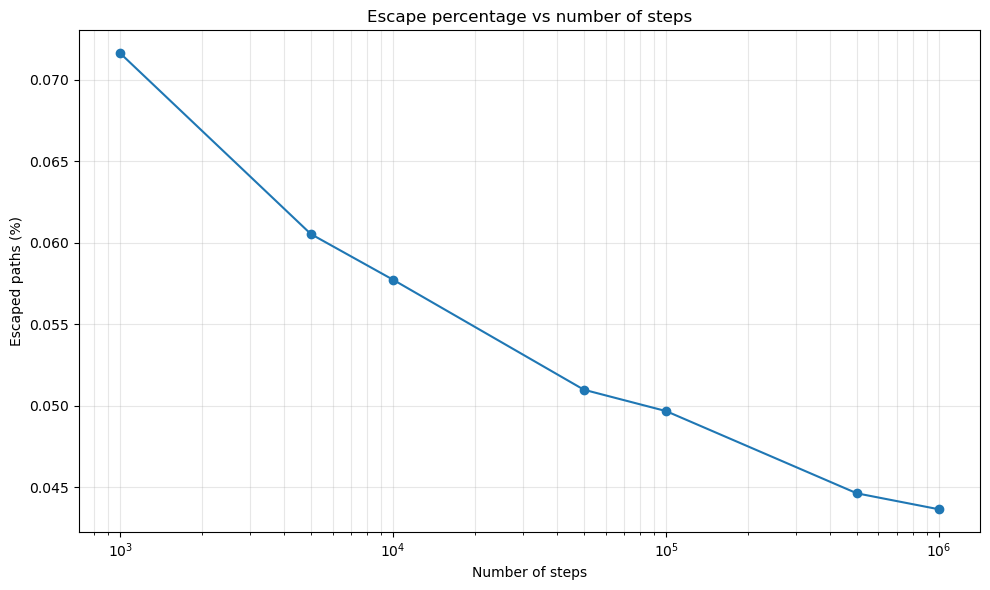
\includegraphics[width=\linewidth]{figures/escape_precentage.png}
    \caption{Escape percentage vs number of steps.}
    \label{fig:escape_percentage}
\end{figure}
\FloatBarrier
The escape percentages in Figure~\ref{fig:escape_percentage} were estimated by Monte Carlo simulation of the Euler-Maruyama scheme for the SDE \eqref{eq:barrier_updated_rep_SDE} where $g(x)=\pi-x$ with initial value $R_0=\pi$, final time $T=100$, and parameters $\mu=\varepsilon=0.01$, so that the diffusion coefficient is $2\sqrt{\varepsilon}=0.2$. For each choice of time discretization, a total of $10^7$ sample paths were simulated. The number of time steps was varied over the logarithmic grid
\[
1,\,5,\,10,\,50,\,100,\,500,\,10^3,\,5\cdot 10^3,\,10^4,\,5\cdot 10^4,\,10^5,\,5\cdot 10^5,\,10^6.
\]
A path was classified as escaped if the numerical approximation satisfied $R_k\leq 0$ or $R_k\geq 2\pi$ at any time step. The implementation was carried out on the GPU using CuPy in single precision (\texttt{float32}), with the total simulation split into batches chosen adaptively from the available GPU memory using a safety factor of $0.85$.

A trend line was originally intended to be added to Figure~\ref{fig:escape_percentage}. However, since the simulations were computationally expensive and the underlying numerical output was not saved, but only the final figure, it was not possible to add such a curve afterwards without rerunning the full experiment.

We observe that the number of escapes decreases as the step size decreases, which is likely because the random noise increments become smaller and therefore have a lower probability of producing a jump large enough to leave the interval.


\begin{figure}[h]
    \centering
    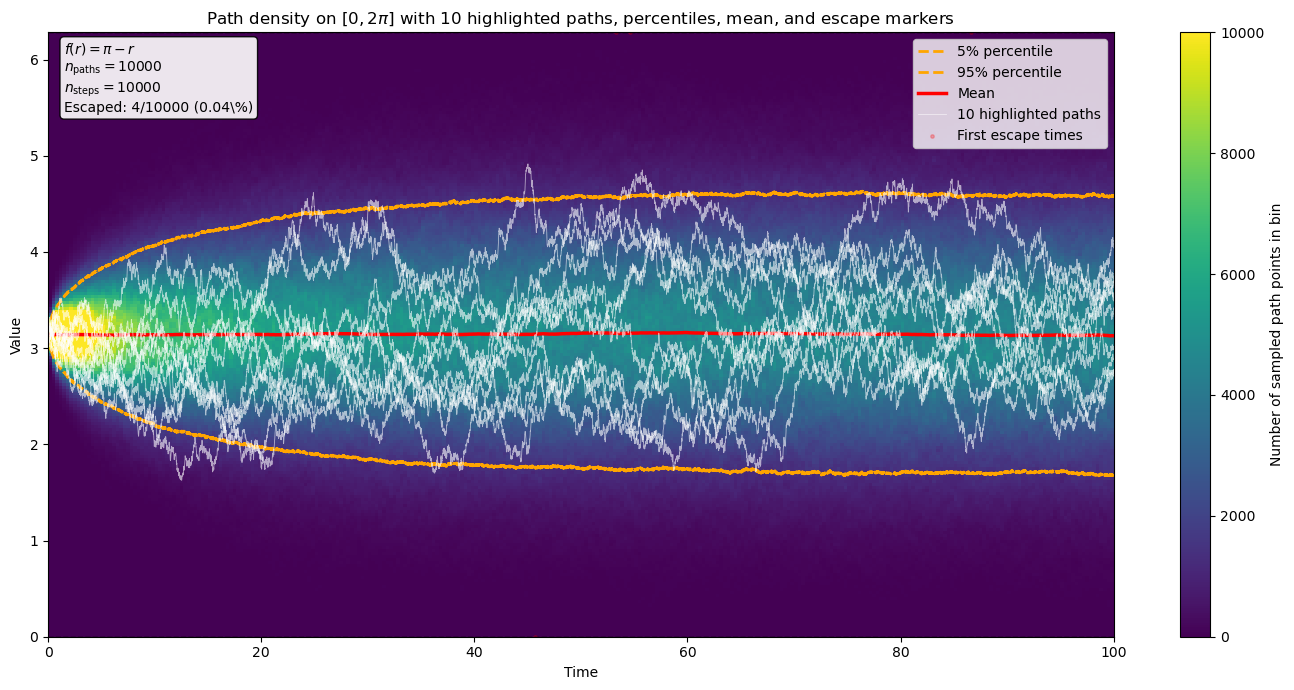
\includegraphics[width=\linewidth]{figures/example_paths.png}
    \caption{Path density on $[0,2\pi]$ with 10 highlighted paths, percentiles, mean, and escape markers.}
    \label{fig:example_paths}
\end{figure}

\FloatBarrier 
Figure~\ref{fig:example_paths} provides a visual example of the simulated dynamics for the Euler-Maruyama approximation of the SDE on the interval $[0,2\pi]$. The background heatmap represents the empirical path density over time based on $10\,000$ simulated paths with $10\,000$ time steps, while the white curves show $10$ selected sample paths. The red curve denotes the empirical mean and the orange curves denote the $5\%$ and $95\%$ empirical percentiles. The figure illustrates that most paths remain concentrated around the center of the interval, while the spread increases over time due to the stochastic forcing. At the same time, a small number of trajectories escape the interval, as indicated by the escape markers, which is consistent with the nonzero escape percentages reported in Figure~\ref{fig:escape_percentage}. In this particular simulation, $4$ out of $10\,000$ paths escaped, corresponding to an escape rate of $0.04\%$.

\subsubsection{Numerical implementation using backward Euler-Maruyama/drift-implicit scheme}
A natural modification of the forward Euler-Maruyama method is the backward Euler-Maruyama, or drift-implicit, scheme. In the present setting, the purpose of this scheme is to replace the explicit drift evaluation used in the forward method by an implicit update, which is better suited to the singular barrier structure of the drift and is expected to prevent escape from the interval.

Following Neuenkirch and Szpruch \cite{neuenkirch2014domain}, the backward Euler-Maruyama, or drift-implicit, scheme is analyzed for additive-noise SDEs on a bounded domain under a one-sided Lipschitz condition on the drift. In particular, they assume that the transformed SDE has a unique strong solution taking values in an interval $(\alpha,\beta)$, and that the drift is continuous and satisfies a one-sided Lipschitz condition. Under an additional regularity assumption, this framework yields strong convergence of order one for the drift-implicit scheme.

In the notation of \cite{neuenkirch2014domain}, Assumption 2.1 is
\[
 -\infty < \alpha < \beta < \infty,\qquad
\text{and SDE (6) has a unique strong solution with } x(t)\in(\alpha,\beta)\ \text{for all } t\ge 0 \ \text{a.s.}
\]
and Assumption 2.2 is
\[
f:(\alpha,\beta)\to(\alpha,\beta)\ \text{is continuous, and there exists } K\in\mathbb{R}
\text{ such that }
(x-y)\bigl(f(x)-f(y)\bigr)\le K|x-y|^2
\]
for all $x,y\in(\alpha,\beta)$ \cite{neuenkirch2014domain}.

In the present setting, the natural codomain is $\mathbb{R}$, and the corresponding form of Assumption 2.2 is therefore
\[
f:(\alpha,\beta)\to\mathbb{R}\ \text{is continuous, and there exists } K\in\mathbb{R}
\text{ such that }
(x-y)\bigl(f(x)-f(y)\bigr)\le K|x-y|^2
\]
for all $x,y\in(\alpha,\beta)$.

By the Feller-test argument above, Assumption 2.1 is satisfied for the barrier SDE on $(0,2\pi)$. It therefore remains to verify Assumption 2.2. For the drift in the relative-distance equation,
\[
f(x)=2\cdot 10^{-2}\Bigl(\pi-x+\frac{1}{x}+\frac{1}{x-2\pi}\Bigr),
\]
and hence
\[
f'(x)=-2\cdot 10^{-2}\Bigl(1+\frac{1}{x^2}+\frac{1}{(x-2\pi)^2}\Bigr).
\]
Using the Mean Value Theorem,
\[
\frac{f(x)-f(y)}{x-y}=f'(c)\qquad \text{for some } c\in(x,y),
\]
and since
\[
f'(c)\le -2\cdot 10^{-2}\qquad \text{for all } c\in(0,2\pi),
\]
it follows that Assumption 2.2 holds. Although this does not by itself yield a convergence rate in the present setting, it shows that the drift-implicit scheme may be well aligned with the singular barrier structure and provides a much more stable numerical update than the forward Euler-Maruyama method.

The backward Euler-Maruyama update for the relative-distance SDE is
\begin{align}
X_{k+1}-f(X_{k+1})\Delta t =X_k+2\sqrt{\varepsilon} \Delta W_{k+1}.
\label{eq:backward-Euler-Maruyama/drift-implicit}
\end{align}
Thus the quantity
\[
X_k+2\sqrt{\varepsilon}\,\Delta W_{k+1}=C
\]
is known at step $k+1$, while the left-hand side defines an implicit scalar equation for $X_{k+1}$. Since the admissible state space is $(0,2\pi)$, each time step amounts to solving
\begin{align}
x-2\mu \Delta t\Bigl(\pi-x+\frac{1}{x}+\frac{1}{x-2\pi}\Bigr)=C.
\label{eq:backward-update-specific}
\end{align}
Writing
\[
k=2\mu \Delta t,
\]
this becomes
\[
x-k\Bigl(\pi-x+\frac{1}{x}+\frac{1}{x-2\pi}\Bigr)=C.
\]
This equation reduces to a cubic polynomial in $x$, and therefore admits a closed-form solution by Cardano's formula. More precisely,
\[
x=
\frac{C+\pi(2+3k)}{3(1+k)}
+\sqrt[3]{-\frac{q}{2}+\sqrt{\Delta}}
+\sqrt[3]{-\frac{q}{2}-\sqrt{\Delta}},
\]
where
\[
q=\frac{2b^3-9abc+27a^2d}{27a^3},
\qquad
\Delta=\left(\frac{q}{2}\right)^2+\left(\frac{p}{3}\right)^3,
\qquad
p=\frac{3ac-b^2}{3a^2},
\]
and
\[
a=1+k,\qquad
b=-\bigl(C+\pi(2+3k)\bigr),\qquad
c=2\pi C+2\pi^2k-2k,\qquad
d=2\pi k.
\]
See Appendix~\ref{sec:closed_form_update} for the derivation. This means that, even though a direct convergence theorem is not established here, the method still has a well-defined update within the admissible interval, and the exact solution remains in that interval almost surely. Together with the fact that the setting comes close to satisfying the framework of \cite{neuenkirch2014domain}, this provides a strong indication that the method may nevertheless exhibit good convergence behavior in practice.


\begin{figure}[h]
    \centering
    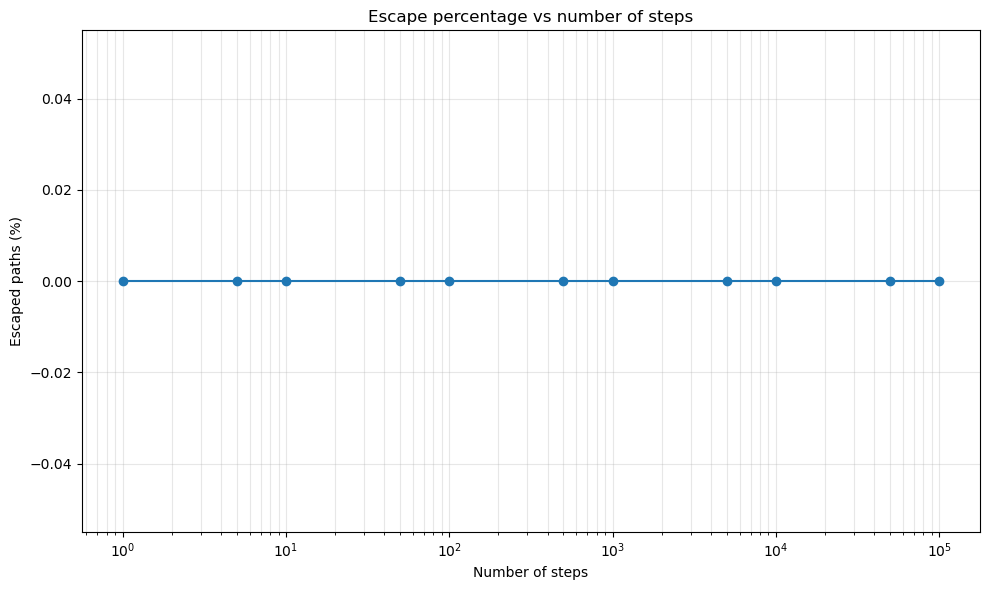
\includegraphics[width=\linewidth]{figures/escape_precentage_backward.png}
    \caption{Escape percentage vs number of steps.}
    \label{fig:escape_percentage_backward}
\end{figure}

In comparison with the forward Euler-Maruyama experiment, the overall simulation setup is unchanged: the same barrier SDE is considered, with $R_0=\pi$, final time $T=100$, and parameters $\mu=\varepsilon=0.01$. The essential difference is that each time step is now computed through the implicit update \eqref{eq:backward-update-specific}, rather than by an explicit drift evaluation. As in the forward case, the escape percentage in Figure~\ref{fig:escape_percentage_backward} was estimated by GPU-based Monte Carlo simulation in CuPy using single precision, batched path generation, and a logarithmic grid of time steps. In the backward implementation, a path is counted as escaped only if the implicit solver fails numerically or returns a value outside $(0,2\pi)$.

\begin{figure}[h]
    \centering
    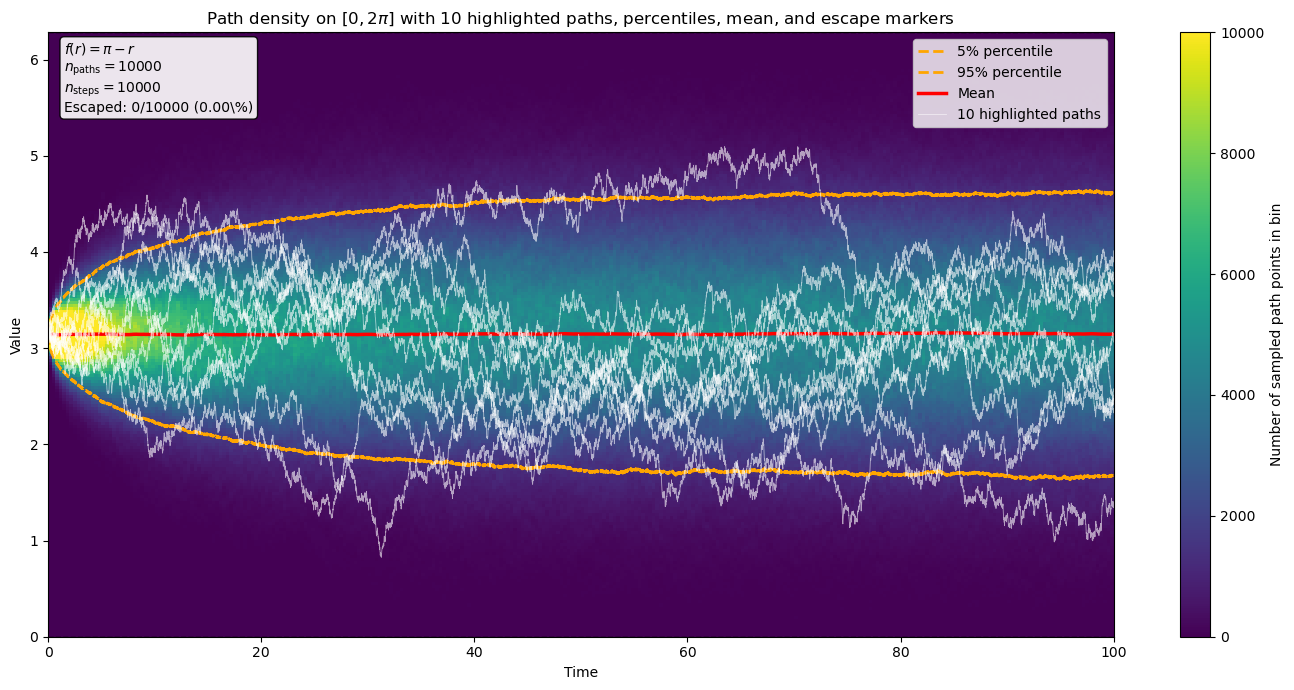
\includegraphics[width=\linewidth]{figures/example_paths_backward.png}
    \caption{Path density on $[0,2\pi]$ with 10 highlighted paths, percentiles, mean, and escape markers.}
    \label{fig:example_paths_backward}
\end{figure}

Figure~\ref{fig:example_paths_backward} provides the corresponding visual example for the drift-implicit method. Relative to the forward Euler-Maruyama plot, the notable difference is that the sampled trajectories remain confined to the interval and no visible escape events occur. This is consistent with the construction of the backward update, which is designed to select the admissible root in $(0,2\pi)$ at every step.

It is therefore observed that, unlike the forward Euler-Maruyama method, the backward Euler-Maruyama or drift-implicit scheme is constructed so that escaping paths do not occur in the numerical experiment. 

However, aside from the escape behavior, the two figures are qualitatively very similar. In both cases, the empirical mean remains close to $\pi$, and the $5\%$ and $95\%$ percentile curves have nearly the same overall shape and spread over time. This indicates that, for the large majority of paths, the backward Euler-Maruyama scheme reproduces the same bulk dynamics as the forward Euler-Maruyama scheme. The main visible difference is therefore not in the central part of the distribution, but in the treatment of trajectories near the boundary. In the forward scheme, a small number of paths eventually leave the interval, whereas in the backward scheme all displayed trajectories remain in $(0,2\pi)$ throughout the simulation. Thus, the drift-implicit method appears to preserve the same overall stochastic behavior while at the same time enforcing the non-escape property that is physically required by the model.

\subsubsection{Direct detialed comparison between standard Euler-Maruyama, clipped Euler-Maruyama and  backward Euler-Maruyama}

To study the numerical behavior of the barrier SDE in greater detail, three first-order discretization schemes are now compared directly: the standard Euler-Maruyama method, a clipped Euler-Maruyama method, and the backward Euler-Maruyama or drift-implicit method. The purpose of this comparison is to move beyond the escape-percentage plots and instead examine how the different schemes approximate qualitative properties of the continuous-time model over time. In particular, the comparison is aimed at assessing stability, preservation of the state constraint, and the extent to which each method respects the symmetry of the dynamics around $\pi$. This provides a more detailed picture of convergence behavior, since a scheme may appear reasonable from path plots alone while still introducing systematic bias in distributional quantities or higher-order moments.

\paragraph{Standard Euler-Maruyama scheme}
\begin{align}
    X_{k+1}=X_{k}+2\mu \Bigl (\pi -X_{k}+\frac{1}{X_{k}}+\frac{1}{X_{k}-2\pi}\Bigr ) \Delta t +2\sqrt{\varepsilon} \Delta W_{k+1}
    \label{eq:standard-Euler-Maruyama}
\end{align}

\paragraph{Clipped Euler-Maruyama scheme}

Where we define $\delta=10^{-30}$ to stop standard Euler-Maruyama scheme to escape $(0,2\pi)$


\begin{align}
    X_{k+1}=\min \Bigl (\max \Bigl (X_{k}+2\mu \Bigl (\pi -X_{k}+\frac{1}{X_{k}}+\frac{1}{X_{k}-2\pi}\Bigr ) \Delta t +2\sqrt{\varepsilon} \Delta W_{k+1} , 2\pi-\delta \Bigr ), \delta \Bigr )
    \label{eq:clipped-Euler-Maruyama}
\end{align}

\paragraph{Backward Euler-Maruyama scheme}

\begin{align}
X_{k+1}-2\mu \Bigl (\pi -X_{k}+\frac{1}{X_{k}}+\frac{1}{X_{k}-2\pi}\Bigr ) \Delta t =X_k+2\sqrt{\varepsilon} \Delta W_{k+1}
\label{eq:backward-Euler-Maruyama/drift-implicit}    
\end{align}

\paragraph{Convergence assessment using oddmoments}

To make the comparison more informative, it is useful to exploit the symmetry of the SDE around $\pi$. Define
\[
Y_t=X_t-\pi.
\]
Since $Y_t$ is obtained from $X_t$ by a translation, It\^o's formula gives
\[
dY_t=dX_t.
\]
Hence the SDE for $Y_t$ becomes
\[
dY_t=2\mu\Bigl(\frac{1}{Y_t+\pi}+\frac{1}{Y_t-\pi}-Y_t\Bigr)dt+2\sqrt{\varepsilon}\,dW_t.
\]
If $Y_0=0$, then the integral form is
\[
Y_t
=
2\mu\int_0^t \Bigl(\frac{1}{Y_s+\pi}+\frac{1}{Y_s-\pi}-Y_s\Bigr)ds
+
2\sqrt{\varepsilon}\int_0^t dW_s.
\]

Now define
\[
Z_t=-Y_t.
\]
Then
\[
dZ_t=-dY_t,
\]
and therefore
\[
d(-Y_t)
=
- \Bigl( 2\mu\Bigl(\frac{1}{-Z_t+\pi}+\frac{1}{-Z_t-\pi}+Z_t\Bigr)dt
+
2\sqrt{\varepsilon}\,dW_t \Bigr).
\]
Rewriting the drift gives
\[
dZ_t
=
2\mu\Bigl(\frac{1}{Z_t-\pi}+\frac{1}{Z_t+\pi}-Z_t\Bigr)dt
-
2\sqrt{\varepsilon}\,dW_t.
\]
Thus
\[
Z_t
=
2\mu\int_0^t \Bigl(\frac{1}{Z_s+\pi}+\frac{1}{Z_s-\pi}-Z_s\Bigr)ds
-
2\sqrt{\varepsilon}\int_0^t dW_s.
\]

Now use the symmetry of Brownian motion:
\[
-2\sqrt{\varepsilon}\int_0^t dW_s \overset{d}{=} 2\sqrt{\varepsilon}\int_0^t dW_s.
\]
It follows that $Y_t$ and $-Y_t$ satisfy the same distributional equation, and hence
\[
Y_t \overset{d}{=} -Y_t.
\]
Therefore
\[
X_t-\pi \overset{d}{=} \pi-X_t.
\]
In particular, for every $k\in\mathbb{N}$,
\[
E[(X_t-\pi)^{2k+1}]=0.
\]
Thus all odd centered moments vanish, which provides a useful quantity for comparing the numerical schemes.

\newpage

\paragraph{Figures and numerical experiment} 

Below are numerical results for the different schemes.
\FloatBarrier

\begin{figure}[h]
    \centering
    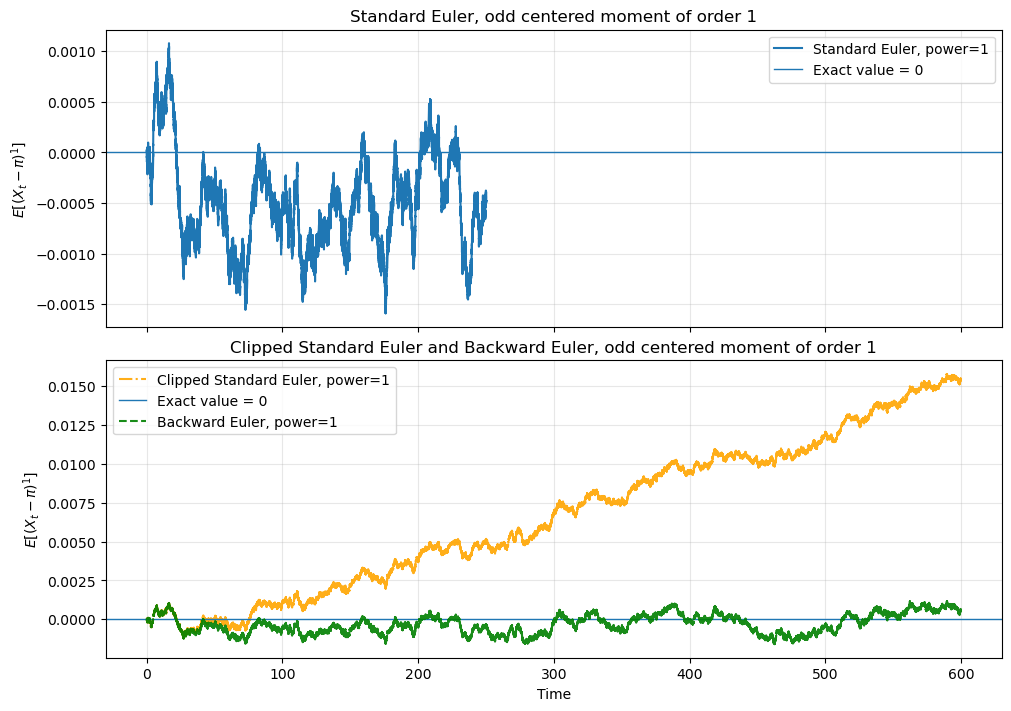
\includegraphics[width=0.95\textwidth]{figures/first_moment_difference.png}
    \caption{Odd centered moment of order $1$. The exact value is $0$. Standard Euler-Maruyama shows noticeable deviation, clipped Euler-Maruyama exhibits a systematic drift, while backward Euler-Maruyama remains close to zero over the full time interval.}
    \label{fig:odd-moment-1}
\end{figure}

\begin{figure}[h]
    \centering
    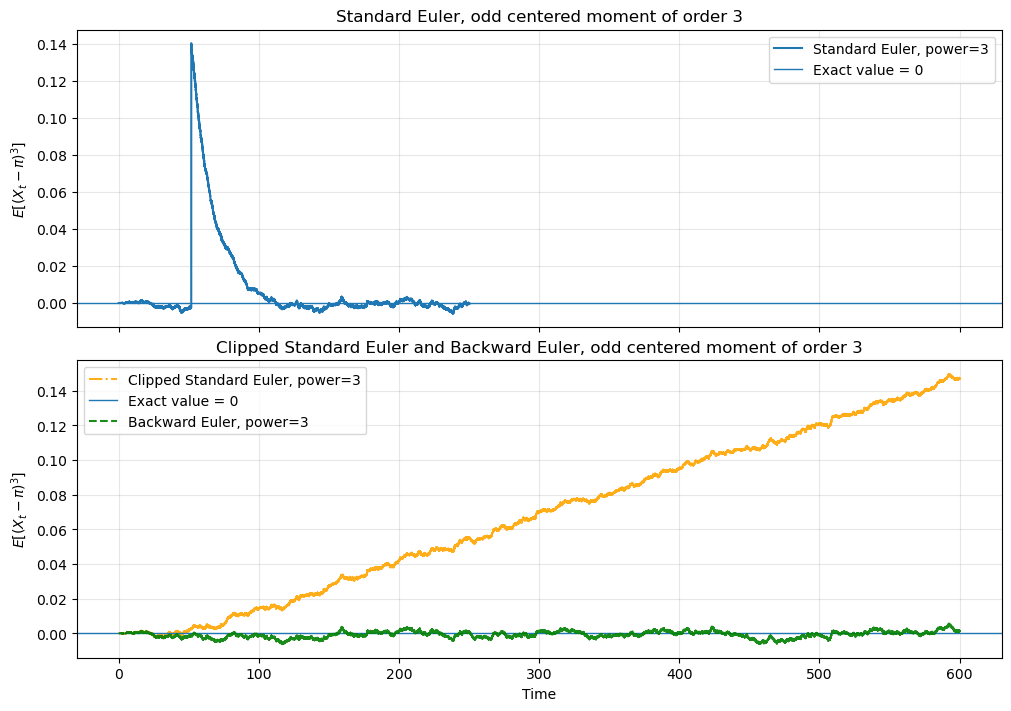
\includegraphics[width=0.95\textwidth]{figures/3thirdmoment_diff.png}
    \caption{Odd centered moment of order $3$. Standard Euler-Maruyama develops a large transient spike, clipped Euler-Maruyama accumulates a persistent positive bias, and backward Euler-Maruyama stays close to the exact value $0$.}
    \label{fig:odd-moment-3}
\end{figure}

\begin{figure}[h]
    \centering
    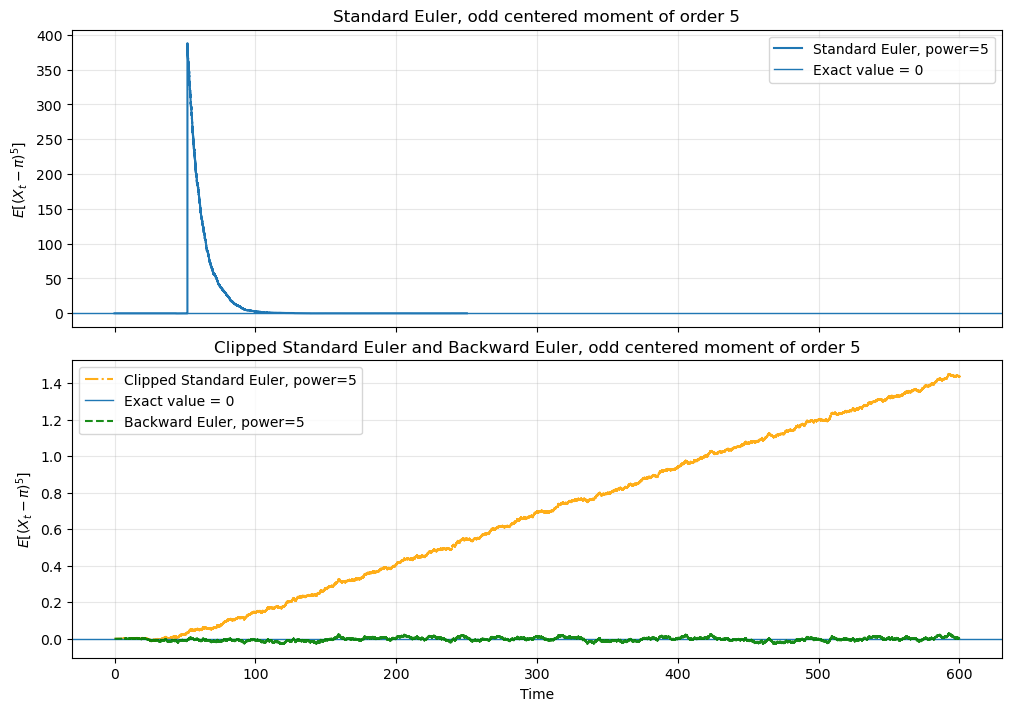
\includegraphics[width=0.95\textwidth]{figures/5moment_diff.png}
    \caption{Odd centered moment of order $5$. The same qualitative pattern becomes even more pronounced for higher moments: standard Euler-Maruyama becomes unstable, clipped Euler-Maruyama introduces a large bias, and backward Euler-Maruyama remains stable and centered around the correct value.}
    \label{fig:odd-moment-5}
\end{figure}

\begin{figure}[h]
    \centering
    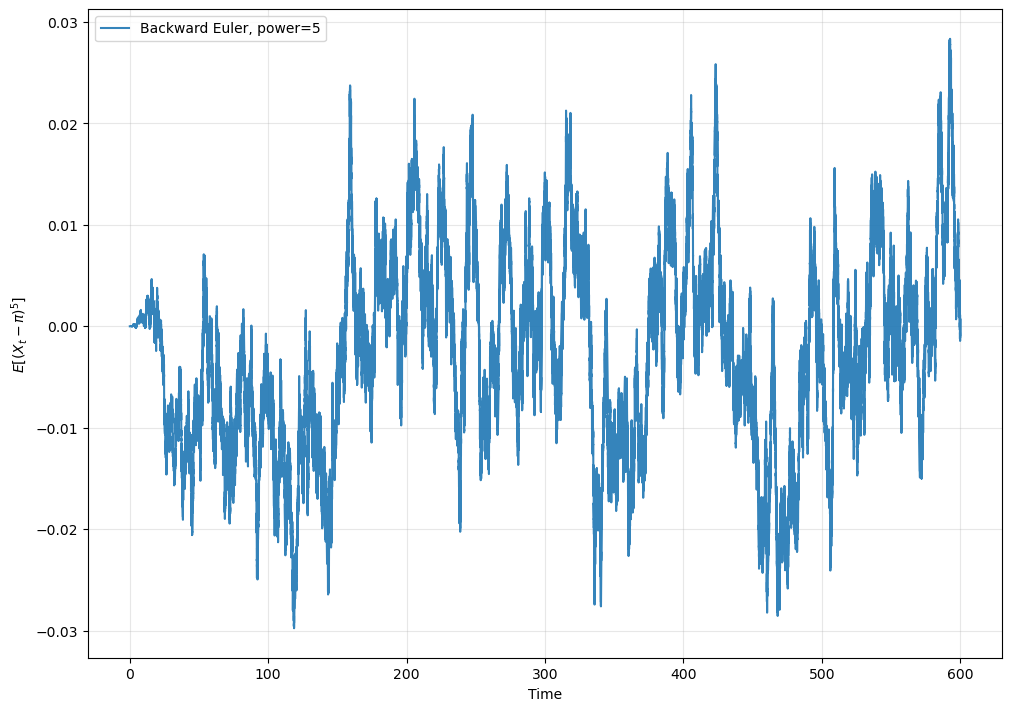
\includegraphics[width=0.95\textwidth]{figures/backward_only_5_moment.png}
    \caption{Backward Euler-Maruyama, odd centered moment of order $5$. The empirical quantity $E[(X_t-\pi)^5]$ fluctuates around the exact value $0$ without any visible systematic drift, which is consistent with preservation of the symmetry around $\pi$.}
    \label{fig:backward-only-moment-5}
\end{figure}

\begin{figure}[h]
    \centering
    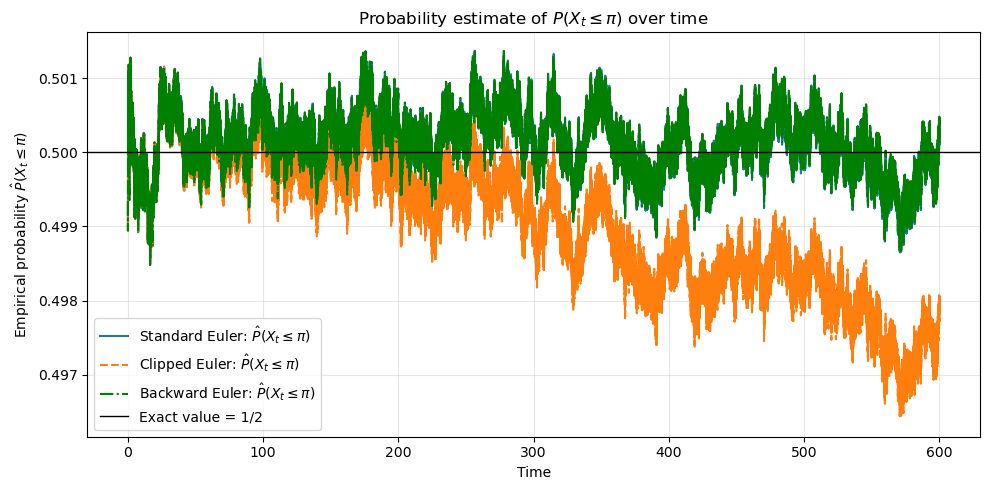
\includegraphics[width=0.95\textwidth]{figures/probability_estimate_over_time.png}
    \caption{Empirical estimate of $\mathbb{P}(X_t \le \pi)$ over time. The exact value is $1/2$ by symmetry. Standard Euler-Maruyama and backward Euler-Maruyama stay close to the exact level, while clipped Euler-Maruyama develops a visible downward bias, indicating that the clipping procedure distorts the invariant symmetry of the dynamics.}
    \label{fig:probability-estimate-over-time}
\end{figure}

\FloatBarrier

The numerical results show a clear qualitative difference between the three schemes. The clipped Euler-Maruyama method develops a systematic positive bias in the odd centered moments, and this bias becomes more pronounced as the order of the moment increases. In particular, Figures~\ref{fig:odd-moment-1}, \ref{fig:odd-moment-3}, and \ref{fig:odd-moment-5} show that the clipped scheme produces a persistent upward drift away from the exact value $0$, while the backward Euler-Maruyama method remains close to zero throughout the simulation horizon. This indicates that clipping prevents escape only by introducing an artificial distortion of the dynamics near the boundary, and that this distortion breaks the symmetry around $\pi$ which the continuous-time model possesses.

The standard Euler-Maruyama method exhibits a different type of failure. In the exact SDE, the solution remains in $(0,2\pi)$ almost surely, so that hitting the singular boundary points is excluded by the continuous-time dynamics. Numerically, however, the situation is different. Since the Gaussian increment $\Delta W_{k+1}$ is unbounded, the explicit update in \eqref{eq:standard-Euler-Maruyama} has a nonzero probability of overshooting the interval in a single time step, no matter how small $\Delta t$ is chosen. Thus, even though the exact process does not hit $0$ or $2\pi$, the numerical scheme can still produce values arbitrarily close to the singularities, and once this happens the drift term becomes extremely large in magnitude. This is precisely what causes the large spikes visible in Figures~\ref{fig:odd-moment-3} and \ref{fig:odd-moment-5}: a very small number of unstable paths can dominate the empirical moment and produce values far from the theoretical value $0$.

This effect is not merely theoretical. The simulations were carried out with
\[
n_{\text{paths}}=10^6
\qquad\text{and}\qquad
n_{\text{steps}}=6\cdot 10^5,
\]
so the total number of updates is extremely large. Consequently, even if the probability of a catastrophic overshoot in a single step is very small, the cumulative probability that such an event occurs somewhere in the simulation is no longer negligible. For this reason, numerical blow-up is observed in practice for the standard Euler-Maruyama scheme.

A natural response would be to remove or kill paths as soon as they leave the interval. However, doing so would itself change the numerical experiment and would no longer provide a fair raw comparison with the unclipped or clipped schemes. In particular, path removal introduces an additional selection mechanism, since the remaining sample no longer represents the original explicit Euler dynamics. For this reason, the instability of the standard Euler-Maruyama method is better interpreted as an inherent defect of the scheme in this singular setting, rather than something that should be corrected by post-processing.

The probability plot in Figure~\ref{fig:probability-estimate-over-time} provides further evidence of this distinction. The backward Euler-Maruyama method remains close to the exact symmetry value $1/2$, whereas the clipped Euler-Maruyama method develops a visible downward drift. In contrast, the standard Euler-Maruyama method remains close to $1/2$, since paths that blow up numerically do so in both directions, to $-\infty$ and $+\infty$, and therefore do not introduce the same systematic bias in the empirical probability estimate; note that, unfortunately, the blue line is barely visible behind the green one. This confirms that the clipping procedure does not merely stabilize the computation, but also alters the invariant structure of the model. Taken together, the figures indicate that the backward Euler-Maruyama scheme is the only one among the three methods that simultaneously preserves the state constraint, avoids numerical explosion, and remains consistent with the symmetry properties of the continuous-time SDE.

\newpage

\paragraph{Convergence assessment using statioanry distrubution}

Another natural way to assess the long-time behavior of the numerical scheme is through the stationary distribution of the SDE. Following the derivation from the lectures, we rewrite our SDE in potential form. Recall that
\[
\dd X_t
=
2\mu\Bigl(\pi-X_t+\frac{1}{X_t}+\frac{1}{X_t-2\pi}\Bigr)\dd t
+
2\sqrt{\varepsilon}\,\dd W_t.
\]
We want to write this as
\[
\dd X_t=-V'(X_t)\dd t+\sqrt{2D}\,\dd W_t.
\]
Since
\[
2\sqrt{\varepsilon}=\sqrt{2D},
\]
we have
\[
D=2\varepsilon.
\]
Moreover, in order to match the drift we need
\[
-V'(x)=2\mu\Bigl(\pi-x+\frac{1}{x}+\frac{1}{x-2\pi}\Bigr),
\]
that is,
\[
V'(x)=-2\mu\Bigl(\pi-x+\frac{1}{x}+\frac{1}{x-2\pi}\Bigr).
\]
Integrating gives
\[
V(x)
=
\mu(x-\pi)^2-2\mu\log x-2\mu\log(2\pi-x)+C,
\qquad x\in(0,2\pi),
\]
where the additive constant $C$ is irrelevant for the stationary density.

Now let $\rho(x,t)$ denote the density of $X_t$. Then the corresponding Fokker-Planck equation is
\[
\frac{\partial \rho}{\partial t}
=
\frac{\partial}{\partial x}
\Bigl(
V'(x)\rho+2\varepsilon \frac{\partial \rho}{\partial x}
\Bigr).
\]
If there exists a stationary density $\rho_\infty(x)$, then it must satisfy
\[
0=
\frac{\partial}{\partial x}
\Bigl(
V'(x)\rho_\infty(x)+2\varepsilon \rho_\infty'(x)
\Bigr).
\]
Assuming zero stationary flux, this becomes
\[
V'(x)\rho_\infty(x)+2\varepsilon \rho_\infty'(x)=0.
\]
Dividing by $\rho_\infty(x)$ gives
\[
V'(x)+2\varepsilon \frac{\rho_\infty'(x)}{\rho_\infty(x)}=0,
\]
and therefore
\[
\frac{\rho_\infty'(x)}{\rho_\infty(x)}
=
-\frac{V'(x)}{2\varepsilon}.
\]
Integrating once more yields
\[
\log \rho_\infty(x)
=
-\frac{V(x)}{2\varepsilon}+c,
\]
so that
\[
\rho_\infty(x)
=
\frac{1}{Z}\exp\!\Bigl(-\frac{V(x)}{2\varepsilon}\Bigr),
\qquad x\in(0,2\pi),
\]
where $Z$ is the normalization constant.

Substituting the explicit expression for $V$ gives
\[
\rho_\infty(x)
=
\frac{1}{Z}
x^{\mu/\varepsilon}(2\pi-x)^{\mu/\varepsilon}
\exp\!\Bigl(-\frac{\mu}{2\varepsilon}(x-\pi)^2\Bigr),
\qquad x\in(0,2\pi).
\]
Thus the exact stationary distribution is explicitly known up to the normalization constant.

\paragraph{Numerical comparison with the stationary distribution}

To assess whether the numerical schemes capture the correct long-time behavior, we compared the empirical distribution of the terminal values against the exact stationary density derived above. In the experiment shown in Figures~\ref{fig:stationary-backward}, \ref{fig:stationary-standard}, and \ref{fig:stationary-clipped}, we used
\[
n_{\mathrm{paths}}=10^6,\qquad
n_{\mathrm{steps}}=10^5,\qquad
T=100,\qquad
\mu=\varepsilon=0.01.
\]
For each scheme, the last simulated value of each path was used as an empirical proxy for a stationary sample. Since the exact stationary law is supported on $(0,2\pi)$, values outside this interval were removed before forming the histogram and computing the Kullback--Leibler divergence. Thus, the comparison below should be interpreted as a comparison of the \emph{remaining in-domain samples} with the exact stationary distribution.

We observe that, once these outlying values are removed, the empirical distributions that remain are already very close to the exact stationary density. In particular, all three histograms almost coincide with the theoretical curve, and the reported Kullback--Leibler divergences are very small. This indicates that the bulk of the sample paths reaches the stationary distribution relatively fast. At the same time, this does \emph{not} mean that the standard and clipped Euler schemes are fully correct in the present singular setting. Rather, it shows that among the paths which remain in the physically admissible region, the long-time distribution is already well captured. The important difference is that the backward Euler-Maruyama scheme achieves this while preserving the state constraint, whereas the other schemes require post-processing through removal of nonphysical values.

\begin{figure}[p]
    \centering
    \captionsetup[subfigure]{font=small}

    \begin{subfigure}{0.72\linewidth}
        \centering
        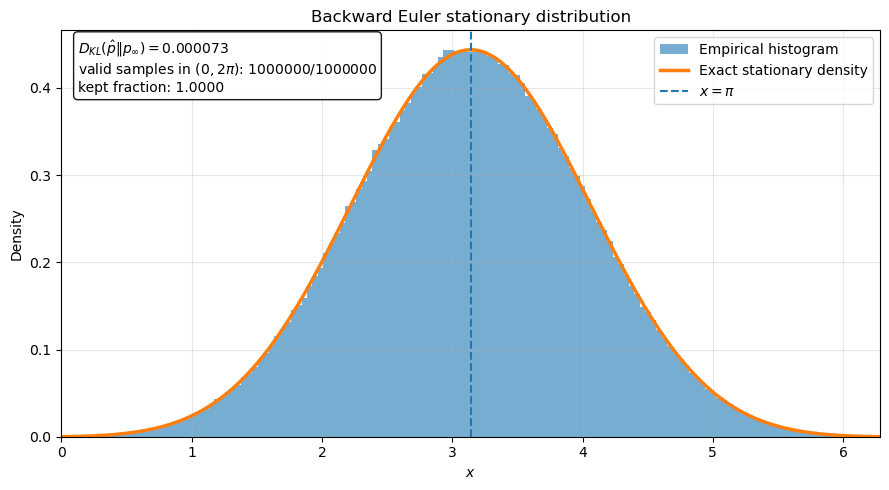
\includegraphics[width=\linewidth]{figures/backward_euler_statioanry.png}
        \caption{Backward Euler-Maruyama stationary distribution.}
        \label{fig:stationary-backward}
    \end{subfigure}

    \vspace{0.4em}

    \begin{subfigure}{0.72\linewidth}
        \centering
        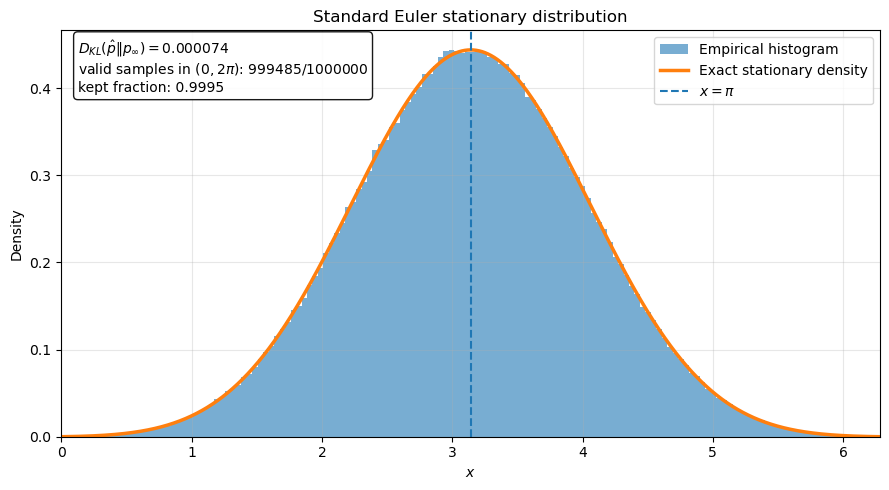
\includegraphics[width=\linewidth]{figures/standard_euler_statioanry.png}
        \caption{Standard Euler-Maruyama stationary distribution.}
        \label{fig:stationary-standard}
    \end{subfigure}

    \vspace{0.4em}

    \begin{subfigure}{0.72\linewidth}
        \centering
        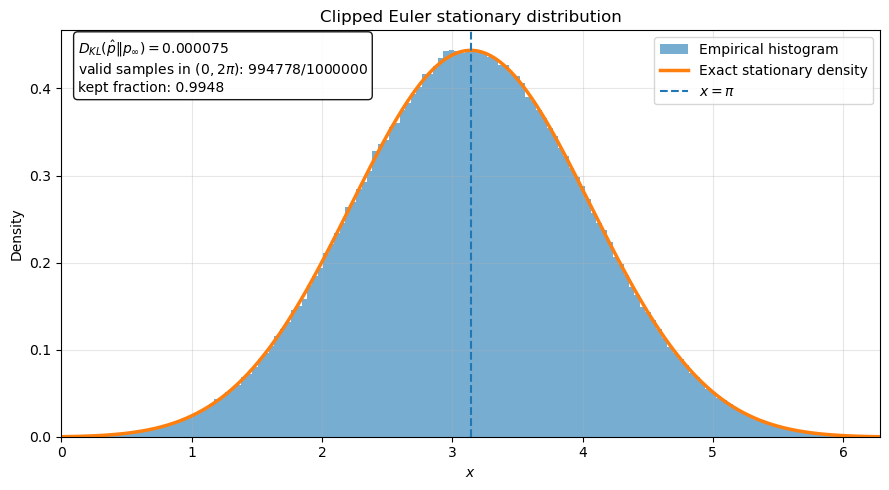
\includegraphics[width=\linewidth]{figures/clipped_euler_stat.png}
        \caption{Clipped Euler-Maruyama stationary distribution.}
        \label{fig:stationary-clipped}
    \end{subfigure}

    \caption{Empirical long-time distributions compared with the exact stationary density. The Kullback--Leibler divergences are very small in all three cases, which indicates that after removing outlying terminal values, the remaining samples are already close to the stationary distribution.}
    \label{fig:stationary-comparison}
\end{figure}

\FloatBarrier

\section{Conclusion}


This project achieved its main goal of constructing a theoretical model that satisfies the physical constraint that particles on the torus do not cross each other. In particular, we derived a barrier-type SDE whose solution remains in the admissible interval almost surely in the simplest case of two particles with no self-propulsion. This gives a rigorous model for the constrained dynamics, which, to the best of our knowledge, was not obtained either numerically in \citet{boffi2024deep} or theoretically even in this simplest setting.

From the numerical point of view, the project also achieved its goal by identifying a relatively efficient method that preserves the correct physical behavior. The backward Euler-Maruyama scheme performed well while maintaining accurate qualitative features of the model. In contrast, the standard Euler-Maruyama method fails because of instability and escape near the singular boundaries, while the ad hoc clipping method introduces a visible bias in several of the qualitative metrics used to assess the viability of the algorithms. This suggests that for this SDE, and for similar singular barrier-type SDEs, a backward method is preferable, especially when the update can be written in explicit form, since this avoids the additional cost of iterative solvers such as Newton's method.

A natural direction for future work is to extend these barrier-type SDE constructions to more complicated interacting systems in higher dimensions. For the present simplified model, the next step would be to establish a rigorous convergence result for the backward scheme. There were some initial attempts in this direction during the project, but the argument did not appear fully correct at the time of writing, and was therefore not included in the report.

%==========================================================
\newpage
% ============================================================

\bibliographystyle{plainnat}
\bibliography{references}


\appendix

\newpage
\section{Derivation of the closed-form update}
\label{sec:closed_form_update}
Consider
\[
x-k\!\left(\frac{1}{x}+\frac{1}{x-\pi}-x\right)=C+k\pi,
\qquad k>0.
\]
Equivalently,
\[
(1+k)x-\frac{k}{x}-\frac{k}{x-\pi}=C+k\pi.
\]
Multiplying by $x(x-\pi)$ gives
\[
(1+k)x^2(x-\pi)-k(x-\pi)-kx=(C+k\pi)x(x-\pi).
\]
Expanding and collecting powers of $x$ yields the cubic equation
\[
(1+k)x^3-\bigl(C+\pi(1+2k)\bigr)x^2+\bigl(C\pi+k\pi^2-2k\bigr)x+k\pi=0.
\]
Thus, with
\[
a=1+k,\qquad
b=-\bigl(C+\pi(1+2k)\bigr),\qquad
c=C\pi+k\pi^2-2k,\qquad
d=k\pi,
\]
we have
\[
ax^3+bx^2+cx+d=0.
\]

Now set
\[
x=y-\frac{b}{3a}.
\]
Then the cubic is transformed into the depressed cubic
\[
y^3+py+q=0,
\]
where
\[
p=\frac{3ac-b^2}{3a^2},
\qquad
q=\frac{2b^3-9abc+27a^2d}{27a^3}.
\]
Hence Cardano's formula gives
\[
y=
\sqrt[3]{-\frac{q}{2}+\sqrt{\Delta}}
+
\sqrt[3]{-\frac{q}{2}-\sqrt{\Delta}},
\qquad
\Delta=\left(\frac{q}{2}\right)^2+\left(\frac{p}{3}\right)^3.
\]
Therefore
\[
x=
-\frac{b}{3a}
+\sqrt[3]{-\frac{q}{2}+\sqrt{\Delta}}
+\sqrt[3]{-\frac{q}{2}-\sqrt{\Delta}}.
\]

Moreover, on the admissible interval $(0,2\pi)$ the left-hand side is strictly increasing, since
\[
\frac{d}{dx}\!\left[x-k\!\left(\frac{1}{x}+\frac{1}{x-\pi}-x\right)\right]
=
1+k+\frac{k}{x^2}+\frac{k}{(x-\pi)^2}>0.
\]
Hence there is exactly one admissible solution in $(0,2\pi)$, and this is the root selected by the update.



\end{document}
